\documentclass[12pt,letterpaper]{article}

\usepackage[utf8]{inputenc}
\usepackage[spanish]{babel}
\usepackage{graphicx}
\usepackage[hidelinks]{hyperref}
\usepackage{hyperref}
\usepackage[left=2cm,right=2cm,top=2.5cm,bottom=2cm]{geometry}
\usepackage{graphicx}
\usepackage{float}
\usepackage{amsmath}
\usepackage{stackrel} 
\usepackage{multicol}
\usepackage{multirow}
\usepackage{fancyhdr}
\usepackage[usenames,dvipsnames,svgnames,table]{xcolor}
\usepackage[document]{ragged2e}
\usepackage{enumerate}

\usepackage{helvet}

\renewcommand{\labelitemi}{$-$}
\renewcommand{\labelitemii}{$\cdot$}
\newcommand\tab[1][1cm]{\hspace*{#1}}

\renewcommand{\familydefault}{\sfdefault}

\definecolor{azul}{RGB}{0,0,255}

\pagestyle{fancy}
\lhead{\begin{picture}(0,0) \put(0,0){
\includegraphics[width=10mm]{./img/logo}} \end{picture}}
\chead{\hspace{1cm}\vspace{0.2cm}Laboratorio 03 - Creando un Cubo Multidimensional con SQL Server Analysis Services}
\rhead{}

\begin{document}
\begin{titlepage}
    \begin{center}
        \begin{figure}[htb]
            \begin{center}
                
\includegraphics[width=3.5cm]{./img/logo}
            \end{center}
        \end{figure}
        \vspace*{0.15in}
        \begin{Large}
            \textbf{UNIVERSIDAD PRIVADA DE TACNA}\\
        \end{Large}
        \vspace*{0.15in}
        \begin{Large}
            \textbf{FACULTAD DE INGENIERÍA} \\
        \end{Large}
        \vspace*{0.1in}
        \begin{Large}
            \textbf{Escuela Profesional de Ingeniería de Sistemas} \\
        \end{Large}
        \vspace*{0.3in}
        \begin{Large}
            \textbf{Laboratorio 03}\\
            \textbf{``Creando un Cubo Multidimensional con SQL Server Analysis Services"}\\
        \end{Large}
        \vspace*{0.2in}
        \begin{Large}
            \textbf{CURSO:} \\
        \end{Large}
        \vspace*{0.1in}
        \begin{large}
            Inteligencia de Negocios\\
        \end{large}
        \vspace*{0.2in}
        \begin{Large}
            \textbf{DOCENTE:} \\
        \end{Large}
        \vspace*{0.1in}
        \begin{large}
            Mag. Patrick Jose Cuadros Quiroga\\
        \end{large}
        \vspace*{0.3in}
        \begin{large}
            \textbf{ALUMNO:} \\
            \begin{flushleft}
                Lipa Calabilla, Abraham  		\hfill	(2019064039) \\
            \end{flushleft}
        \end{large}
        \vspace*{1.3in}
        \begin{large}
            Tacna - Perú\\
        \end{large}
        \vspace*{0.1in}
        \begin{large}
            2022\\
        \end{large}
    \end{center}
\end{titlepage}
\include{Secciones/articulo}
\newpage
\tableofcontents
\justify
\newpage
\begin{LARGE}
    \begin{center}
        \textbf{CREANDO UN CUBO MULTIDIMENSIONAL CON SQL SERVER ANALYSIS SERVICES} \\
    \end{center}
\end{LARGE}
\section{OBJETIVOS}
\begin{itemize}
    \item Crear un cubo Multidimensional, para lo cual se tiene que haber instalado antes el motor de Analysis Services Multidimensional se necesita una base de datos para la creación del cubo, para lo que se necesitaría tener restaurada la base de datos Adventure Works DW.
\end{itemize}

\section{REQUERIMIENTOS}
\begin{itemize}
    \item Conocimientos\\
          Para el desarrollo de esta práctica se requerirá de los siguientes conocimientos básicos:
          \begin{itemize}
              \item Conocimientos básicos de administración de base de datos Microsoft SQL Server.
              \item Conocimientos básicos de Visual Studio 2019.
          \end{itemize}
    \item Software\\
          Así mismo se necesitan los siguientes aplicativos:
          \begin{itemize}
              \item SQL Server Integration Services
              \item Base de datos Adventure Work (OLTP Y Datawarehouse) y AdventureWorksLT2012
              \item Microsoft SQL Server 2016 o superior
              \item Visual Studio 2019
          \end{itemize}
\end{itemize}

\section{CONSIDERACIONES INICIALES}
\begin{itemize}
    \item Tener todos los componentes considerados en los requerimientos de modo que se puedan crear Integration Services Projects
\end{itemize}

\newpage
\section{DESARROLLO}

Abrir el SQL Server Data Tools y dirigirnos a la pestaña de Business Intelligence -> Analysis Services. Como se creará un Modelo Multidimensional desde 0 , seleccionaremos la primera opción. En la casilla de Name le colocamos un nombre al proyecto y a la solución:

\begin{center}
    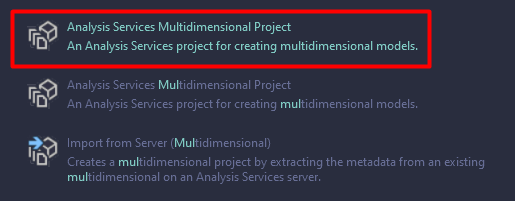
\includegraphics[width=13cm]{./img/img1.png}
\end{center}

\subsection{1. Creación de un Data Source}

En el Solution Explorer nos ubicamos en Data Sources y click derecho, seleccionando la opción de New
Data Source ...

\begin{center}
    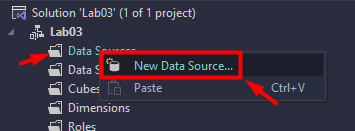
\includegraphics[width=8cm]{./img/img2.png}
\end{center}

Se nos abrirá una ventana de resumen. Click en Next. Si es la primera vez que realizamos un proyecto de estos, no tendremos creadas conexiones. Click en New para crear una nueva conexión hacia la base de datos Adventure Works DW:

\begin{center}
    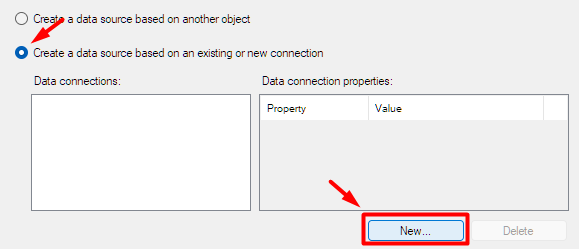
\includegraphics[width=13cm]{./img/img3.png}
\end{center}

Colocamos el nombre del Server donde se ubica la base de datos, en mi caso como es local coloco “.” ,indicándole que es localhost. Ingresamos las credenciales y la base de datos Adventure Works DW 2014. Luego Click en Ok:

\begin{center}
    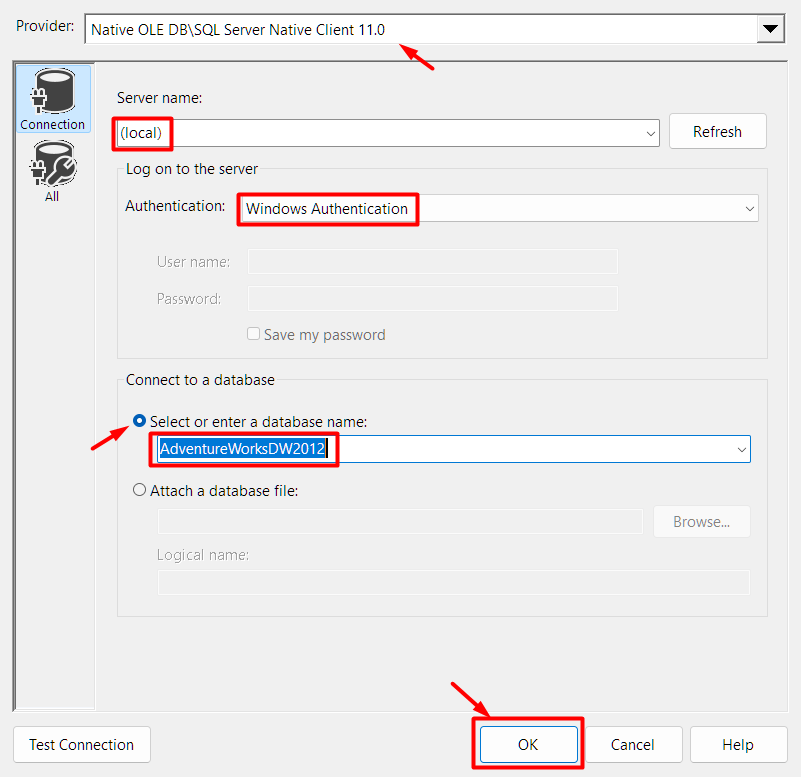
\includegraphics[width=13cm]{./img/img4.png}
\end{center}

Si todo está bien nos aparecerá la conexión creada en la sección de Data connections. Hacemos clic en Finish.

\begin{center}
    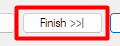
\includegraphics[width=5cm]{./img/img5.png}
\end{center}

\subsection{2. Creación de un Data Source View}

En el Solution Explorer nos ubicamos en Data Sources View y click derecho, seleccionando la opción de New Data Source View ...

\begin{center}
    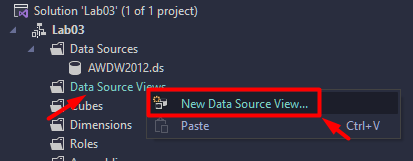
\includegraphics[width=10cm]{./img/img6.png}
\end{center}

Aquí nos aparecerán todos los Data Sources creados en la proyecto, en mi caso nos aparece el creado en la sección 1.

\begin{center}
    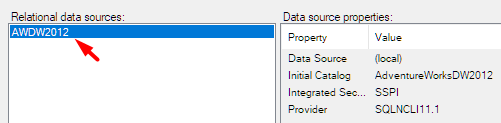
\includegraphics[width=13cm]{./img/img7.png}
\end{center}

Click en Next:

\begin{center}
    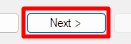
\includegraphics[width=5cm]{./img/img8.png}
\end{center}

Si bien es cierto hemos creado una conexión hacia Adventure Works DW, solo trabajaremos con algunas tablas. Seleccionamos las tablas DimDate,DimProduct y FactInternetSales:

\begin{center}
    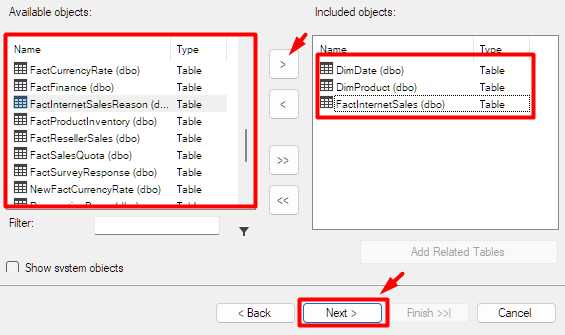
\includegraphics[width=13cm]{./img/img9.png}
\end{center}

Click en Next. Colocamos un nombre el Data Source View creado y click en Finish:

\begin{center}
    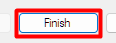
\includegraphics[width=5cm]{./img/img10.png}
\end{center}

Si todo va bien visualizaremos las tablas seleccionadas en el Data Source View:

\begin{center}
    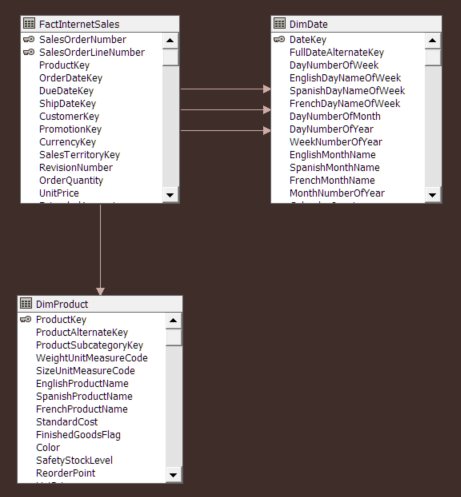
\includegraphics[width=10cm]{./img/img11.png}
\end{center}

\subsection{3. Creación de un Cubo}

En el Solution Explorer nos ubicamos en Cubes y click derecho, seleccionando la opción de New Cube ...

\begin{center}
    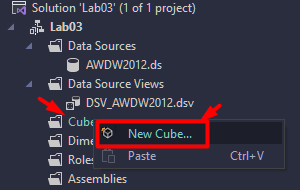
\includegraphics[width=8cm]{./img/img12.png}
\end{center}

Para la creación de un cubo tenemos varias opciones.


Use existing tables: Utilizar tablas del Data Source View.
Create an empty cube: Crear un cubo vacío.
Generate tables in the data source: Nos da la opción de crear tablas a partir de templates.


En este caso utilizaremos las tablas seleccionadas en el Data Source View creada en la sección 2:

\begin{center}
    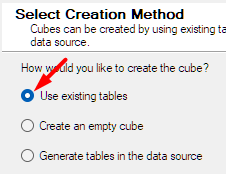
\includegraphics[width=8cm]{./img/img13.png}
\end{center}

Click en Next. Aquí seleccionaremos la FactTable (Tablas de Hechos) , en este caso ubicamos FactInternetSales:

\begin{center}
    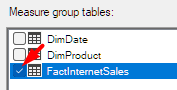
\includegraphics[width=8cm]{./img/img14.png}
\end{center}

Click en Next. Automáticamente el Data Tools identificará todos los campos numéricos y los marcará como candidatos a ser medidas. Podemos observar que inclusive marca los campos utilizados como Foreign Keys. En este caso, seleccionamos solo Order Quantity y Sales Amount:

\begin{center}
    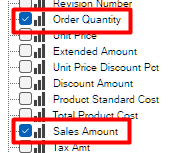
\includegraphics[width=6cm]{./img/img15.png}
\end{center}

Click en Next.
Aquí seleccionamos las dimensiones por las cuales será analizada la data. Inclusive el Data Tools te indica que podría tomar la misma FactTable como Dimensión. Seleccionamos Dim Date y Dim Product:

\begin{center}
    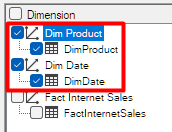
\includegraphics[width=6cm]{./img/img16.png}
\end{center}

Click en Next. Colocamos un nombre el cubo. Hacemos clic en Finish:

\begin{center}
    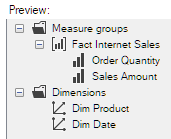
\includegraphics[width=7cm]{./img/img17.png}
\end{center}

\subsection{Procesar Cubo}

En el Solution Explorer nos ubicamos en el nuevo cubo creado CubeSales y click derecho, seleccionando la opción de Process ...

\begin{center}
    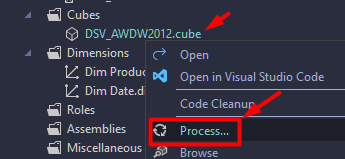
\includegraphics[width=10cm]{./img/img18.png}
\end{center}

Click en Yes

\begin{center}
    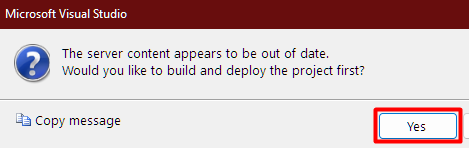
\includegraphics[width=10cm]{./img/img19.png}
\end{center}

Si todo va bien nos mostrará algo como lo siguiente:

\begin{center}
    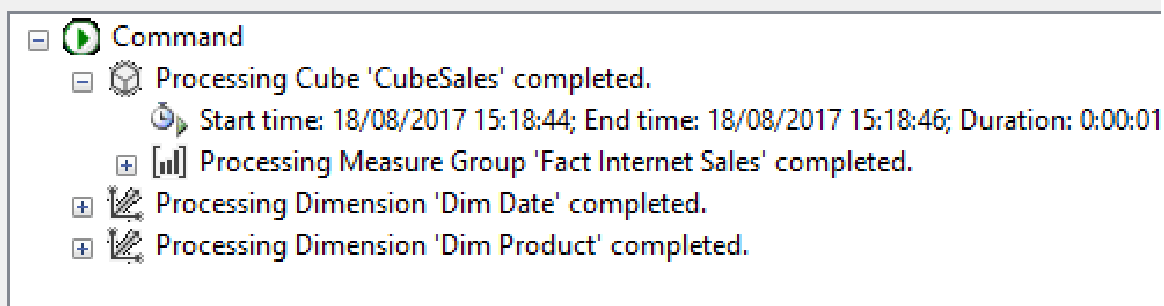
\includegraphics[width=8cm]{./img/img20.png}
\end{center}

Para verificar que nuestros datos se procesaron de forma correcta , en el cubo CubeSales nos dirigimos a la pestaña de Browse:

\begin{center}
    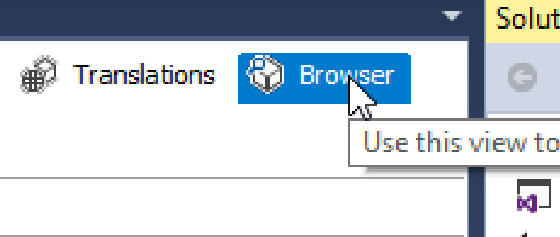
\includegraphics[width=8cm]{./img/img21.png}
\end{center}

En la pestaña de CubeSales, podemos tener un vistazo de las medidas y dimensiones. Arrastramos las columnas de la Fact y la Dimensión Product obteniendo algo como:

\begin{center}
    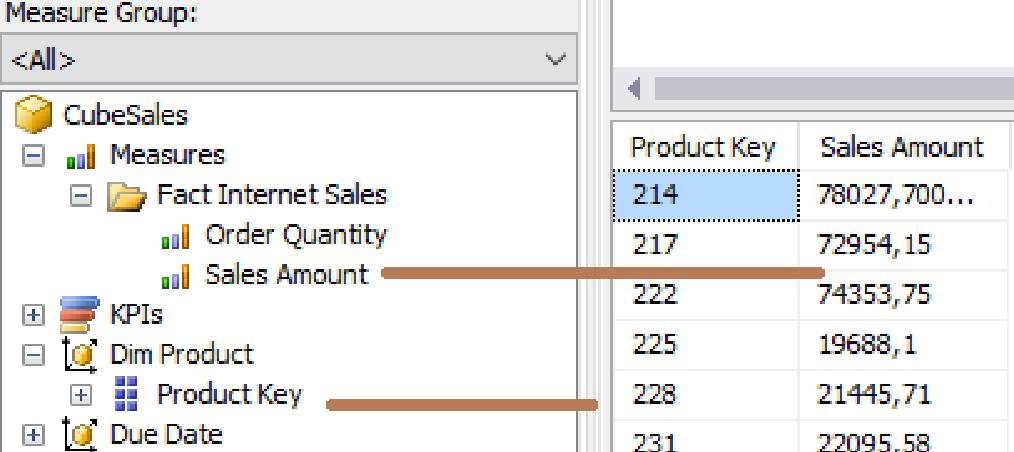
\includegraphics[width=8cm]{./img/img22.png}
\end{center}

\newpage
\section{CONCLUSIONES}
\begin{itemize}
    \item Se creó la conexión necesaria para que se pueda agregar la fuente del cubo
    \item Se creó un cubo teniendo en cuenta las dimensiones requeridas
\end{itemize}
\end{document}